
\documentclass[a4paper,11pt]{article}
\usepackage[a4paper, margin=8em]{geometry}

% usa i pacchetti per la scrittura in italiano
\usepackage[french,italian]{babel}
\usepackage[T1]{fontenc}
\usepackage[utf8]{inputenc}
\frenchspacing 

% usa i pacchetti per la formattazione matematica
\usepackage{amsmath, amssymb, amsthm, amsfonts}

% usa altri pacchetti
\usepackage{gensymb}
\usepackage{hyperref}
\usepackage{standalone}

% imposta il titolo
\title{Appunti Elettronica Digitale}
\author{Luca Seggiani}
\date{2026}

% imposta lo stile
% usa helvetica
\usepackage[scaled]{helvet}
% usa palatino
\usepackage{palatino}
% usa un font monospazio guardabile
\usepackage{lmodern}

\renewcommand{\rmdefault}{ppl}
\renewcommand{\sfdefault}{phv}
\renewcommand{\ttdefault}{lmtt}

% disponi il titolo
\makeatletter
\renewcommand{\maketitle} {
	\begin{center} 
		\begin{minipage}[t]{.8\textwidth}
			\textsf{\huge\bfseries \@title} 
		\end{minipage}%
		\begin{minipage}[t]{.2\textwidth}
			\raggedleft \vspace{-1.65em}
			\textsf{\small \@author} \vfill
			\textsf{\small \@date}
		\end{minipage}
		\par
	\end{center}

	\thispagestyle{empty}
	\pagestyle{fancy}
}
\makeatother

% disponi teoremi
\usepackage{tcolorbox}
\newtcolorbox[auto counter, number within=section]{theorem}[2][]{%
	colback=blue!10, 
	colframe=blue!40!black, 
	sharp corners=northwest,
	fonttitle=\sffamily\bfseries, 
	title=~\thetcbcounter: #2, 
	#1
}

% disponi definizioni
\newtcolorbox[auto counter, number within=section]{definition}[2][]{%
	colback=red!10,
	colframe=red!40!black,
	sharp corners=northwest,
	fonttitle=\sffamily\bfseries,
	title=~\thetcbcounter: #2,
	#1
}

% U.D.M
\newcommand{\amp}{\ensuremath{\mathrm{A}}}
\newcommand{\volt}{\ensuremath{\mathrm{V}}}
\newcommand{\meter}{\ensuremath{\mathrm{m}}}
\newcommand{\second}{\ensuremath{\mathrm{s}}}
\newcommand{\farad}{\ensuremath{\mathrm{F}}}
\newcommand{\henry}{\ensuremath{\mathrm{H}}}
\newcommand{\siemens}{\ensuremath{\mathrm{S}}}

% circuiti
\usepackage{circuitikz}
\usetikzlibrary{babel}

% disegni
\usepackage{pgfplots}
\pgfplotsset{width=10cm,compat=1.9}

% disponi codice
\usepackage{listings}
\usepackage[table]{xcolor}

\definecolor{codegreen}{rgb}{0,0.6,0}
\definecolor{codegray}{rgb}{0.5,0.5,0.5}
\definecolor{codepurple}{rgb}{0.58,0,0.82}
\definecolor{backcolour}{rgb}{0.95,0.95,0.92}

\lstdefinestyle{codestyle}{
		backgroundcolor=\color{black!5}, 
		commentstyle=\color{codegreen},
		keywordstyle=\bfseries\color{magenta},
		numberstyle=\sffamily\tiny\color{black!60},
		stringstyle=\color{green!50!black},
		basicstyle=\ttfamily\footnotesize,
		breakatwhitespace=false,         
		breaklines=true,                 
		captionpos=b,                    
		keepspaces=true,                 
		numbers=left,                    
		numbersep=5pt,                  
		showspaces=false,                
		showstringspaces=false,
		showtabs=false,                  
		tabsize=2
}

\lstdefinestyle{shellstyle}{
		backgroundcolor=\color{black!5}, 
		basicstyle=\ttfamily\footnotesize\color{black}, 
		commentstyle=\color{black}, 
		keywordstyle=\color{black},
		numberstyle=\color{black!5},
		stringstyle=\color{black}, 
		showspaces=false,
		showstringspaces=false, 
		showtabs=false, 
		tabsize=2, 
		numbers=none, 
		breaklines=true
}

\lstdefinelanguage{javascript}{
	keywords={typeof, new, true, false, catch, function, return, null, catch, switch, var, if, in, while, do, else, case, break},
	keywordstyle=\color{blue}\bfseries,
	ndkeywords={class, export, boolean, throw, implements, import, this},
	ndkeywordstyle=\color{darkgray}\bfseries,
	identifierstyle=\color{black},
	sensitive=false,
	comment=[l]{//},
	morecomment=[s]{/*}{*/},
	commentstyle=\color{purple}\ttfamily,
	stringstyle=\color{red}\ttfamily,
	morestring=[b]',
	morestring=[b]"
}

% disponi sezioni
\usepackage{titlesec}

\titleformat{\section}
	{\sffamily\Large\bfseries} 
	{\thesection}{1em}{} 
\titleformat{\subsection}
	{\sffamily\large\bfseries}   
	{\thesubsection}{1em}{} 
\titleformat{\subsubsection}
	{\sffamily\normalsize\bfseries} 
	{\thesubsubsection}{1em}{}

% disponi alberi
\usepackage{forest}

\forestset{
	rectstyle/.style={
		for tree={rectangle,draw,font=\large\sffamily}
	},
	roundstyle/.style={
		for tree={circle,draw,font=\large}
	}
}

% disponi algoritmi
\usepackage{algorithm}
\usepackage{algorithmic}
\makeatletter
\renewcommand{\ALG@name}{Algoritmo}
\makeatother

% disponi numeri di pagina
\usepackage{fancyhdr}
\fancyhf{} 
\fancyfoot[L]{\sffamily{\thepage}}

\makeatletter
\fancyhead[L]{\raisebox{1ex}[0pt][0pt]{\sffamily{\@title \ \@date}}} 
\fancyhead[R]{\raisebox{1ex}[0pt][0pt]{\sffamily{\@author}}}
\makeatother

\begin{document}
% sezione (data)
\section{Lezione del 13-04-26}

% stili pagina
\thispagestyle{empty}
\pagestyle{fancy}

% testo
Finora abbiamo visto il transistore BJT impiegato in circuiti amplificatori \textit{invertenti}, nella cosiddetta configurazione ad \textit{emettitore comune}.

Vediamo adesso una configurazione alternativa a questa.

\subsection{Configurazione a collettore comune}
La configurazione a \textbf{collettore comune} (o a \textit{inseguitore di emettitore}) del transistor BJT è una configurazione alternativa per i circuiti amplificatori col BJT, realizzata come segue:

\begin{center}
\begin{circuitikz}
	\draw
(0,0) node[ground]{} to[R=$R_2$] (0,3)
to[R=$R_1$] (0,6) node[vcc]{};

\draw (0,3) -- (2,3);

\draw (2,3) node[npn, anchor=B] (Q1) {};

\draw (Q1.C) to[short] ++(0,3) node[vcc]{};
\draw (Q1.E) to[R=$R_E$] ++(0,-3) node[ground]{};

\draw[->] (1.2,3.3) -- (1.8,3.3) node[midway, above]{$I_B$};
\draw[->] (Q1.C) ++(0.3,0.5) -- ++(0,-1) node[midway, right]{$I_C$};
\draw[->] (Q1.E) ++(0.3,0) -- ++(0,-.8) node[midway, right]{$I_E$};

\node[ground] at(-4, 0) {};
\draw (-4, 0) to [ sinusoidal voltage source, v=$V_s$] (-4,3)
	to [resistor, l=$R_s$] (-2, 3)
	to [capacitor, l=$C_s$] (0, 3);

\node[ground] at(6, 0) {};
\draw(3, 2.5) to[ capacitor, l=$C_L$] (6, 2.5)
	to[resistor, l=$R_L$] (6, 0);
\end{circuitikz}
\end{center}

Notiamo quindi che la tensione di uscita si va a calcolare sul carico $R_L$, all'emettitore del transistor anziché il collettore.

\subsubsection{Analisi AC}
Assumendo $h_{re} = 0$ e $h_{oe} = 0$ e facendo l'analisi del circuito in AC, si ottiene il seguente circuito (cortesia della collega Rajy):
\begin{center}
	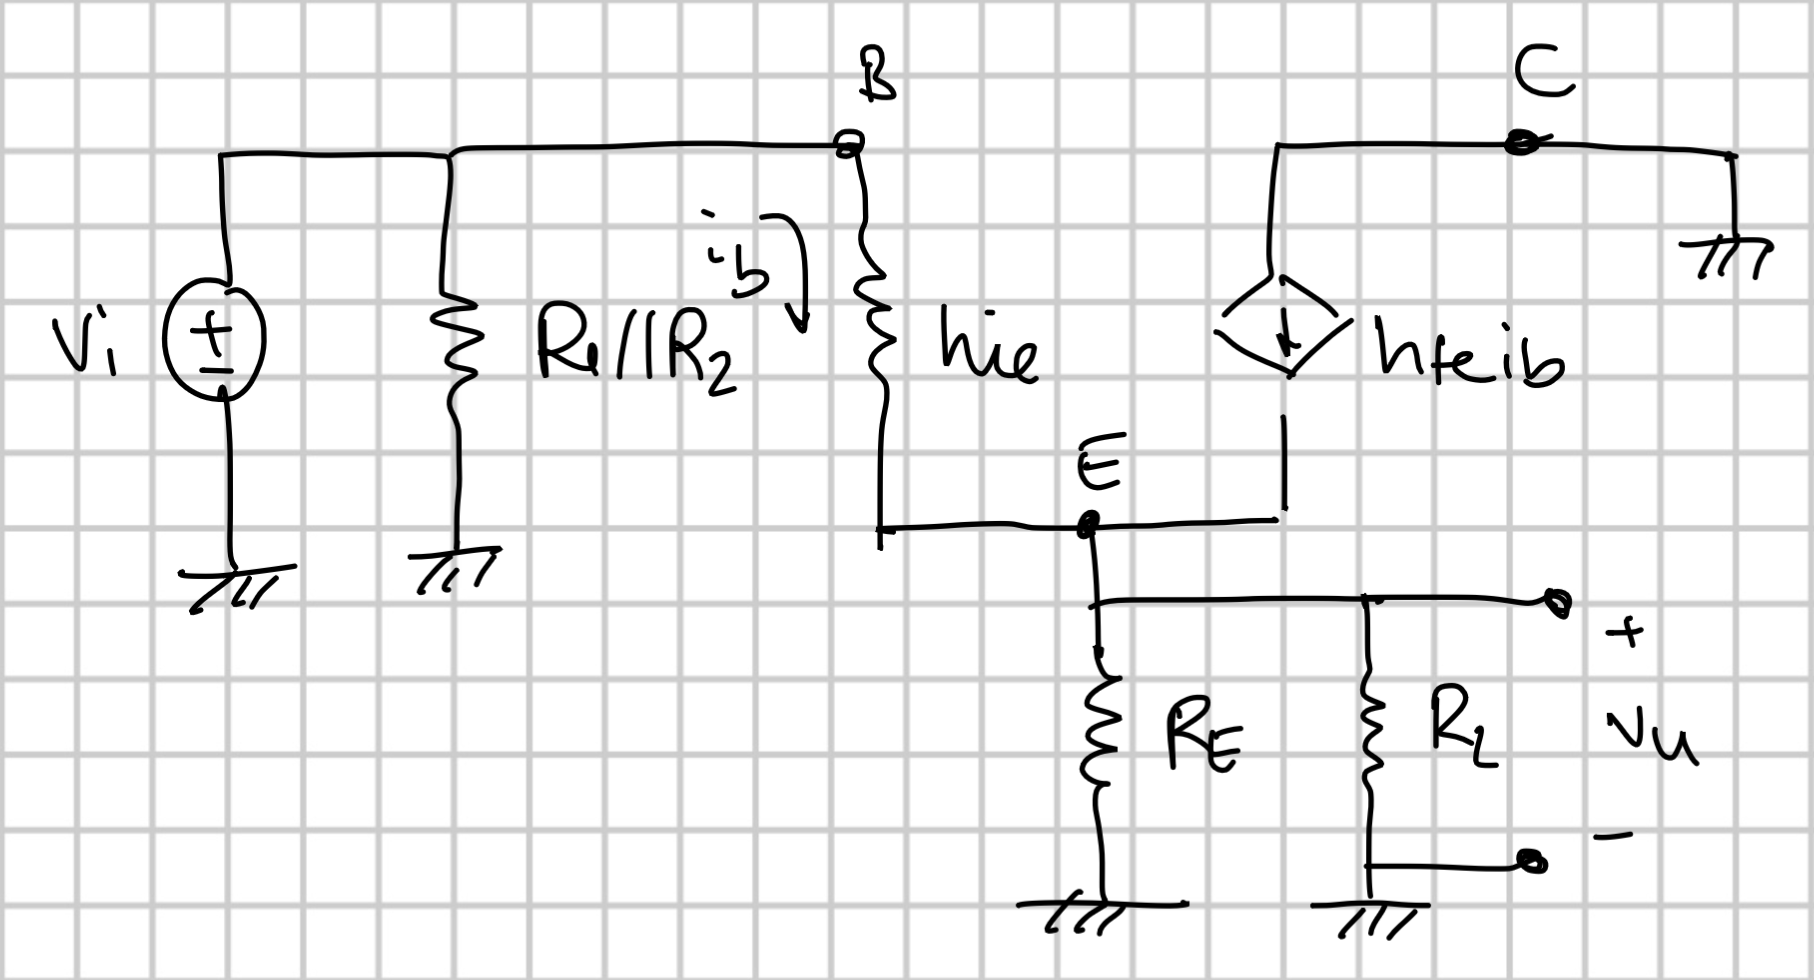
\includegraphics[scale=0.25]{../figures/common_coll_imane.png}
\end{center}

Come sempre, ci interesserà calcolare i parametri $R_I$ e $R_O$ (resistenza in ingreso e in uscita della rete) e $A_I$ e $A_V$ guadagni rispettivamente in corrente e in tensione.

\begin{itemize}
	\item \textbf{\textsf{Guadagno di corrente $A_i$}} \\
Il guadagno di corrente si calcolerà dal rapporto fra la corrente in uscita e quela in entrata. Essendo la corrente $i_o$ in uscita somma negativa della corrente di base e del contributo del generatore dipendente, presa entrante nel BJT, questo sarà semplicemente:
$$
A_i = \frac{i_o}{i_i} = -(h_{fe} + 1)
$$

	\item \textbf{\textsf{Guadagno di tensione $A_v$}} \\
Il guadagno di tensione sarà il rapporto fra la tensione in entrata e quella che imponiamo ai capi del carico $R_L$ (preso aperto). Scriviamo prima di tutto la tensione all'ingresso come:
$$
V_i = h_{ie} i_b + R_E (h_{fe} + 1) i_b
$$
e la tensione al'uscita come semplicemente:
$$
V_u = R_E i_e = R_E (h_{fe} + 1) i_b
$$
Il calcolo viene quindi:
$$
A_v = \frac{V_u}{V_i} = \frac{R_E (h_{fe} + 1) i_b}{(h_{ie} + R (h_{fe} + 1)) i_b}
= \frac{R_E (h_{fe} + 1)}{h_{ie} + R_E (h_{fe} + 1)}
$$

Notiamo a questo punto alcune cose fondamentali:
\begin{enumerate}
	\item Innanzitutto questo amplificatore è \textit{non invertente}, in quanto il segno dell'amplificazione di tensione è positivo;
	\item Allo stesso tempo, non è un amplificatore di tensione in quanto il valore di $A_v$ è per forza minore di $1$ (solitamente è $\sim 1$). Nonostante ciò, il guadagno in corrente è $> 0$, per cui si ha comunque un'amplificazione di \textit{potenza};
	\item Il fatto che la $h_{ie}$ è piccola, come abbiamo anticipato nel punto precedente, significa che $A_v$ è $\sim 1$, per cui la tensione all'emettitore è circa la tensione alla base. Per questo il dispositivo viene detto anche \textit{inseguitore di emettitore}, e ci permette di ottenere un trasferimento di tensione senza attenuazione. Reti di questo tipo ci torneranno utili in seguito come \textit{buffer}, in particolare quando parleremo dei circuiti digitali o degli amplificatori operazionali. 
\end{enumerate}

	\item \textbf{\textsf{Impedenza in uscita $R_o$}} \\
Per la $R_o$, consideriamo ciò che si ottiene all'uscita dell'emettitore del BJT (quindi ignorando $R_E$ e $R_L$), e disattivando il generatore di segnale. In questo caso il parallelo $R_1 || R_2$ non dà contributo, in quanto collegato a massa da entrambi i lati. La tensione all'emettitore sarà allora:
$$
V_p = - h_{ie} i_b
$$
cioè si ha il solo contributo di $h_{ie}$, mentre la corrente che \textit{entra} nell emettitore sarà data sia da $i_b$ che dal generatore pilotato:
$$
i_p = -i_b - h_{fe} i_b = -(h_{fe} + 1) i_b
$$
per cui si ottiene:
$$
R_o = \frac{V_p}{i_p} = \frac{ - h_{ie} i_b }{ - (h_{fe} + 1) i_b } = \frac{h_{ie}}{h_{fe} + 1}
$$
Possiamo chiamare anche questa una legge di \textit{riflessione della resistenza}, stavolta da base a emettitore anziché da emettitore a base.

Notiamo quindi che in questa configurazione (a collettore comune) vale $R_I >> R_O$, in quanto in generale $h_{ie}$ è più piccola delle altre resistenze nel circuito.

	\item \textbf{\textsf{Impedenza in ingresso $R_i$}} \\
Per quanto riguarda la $R_i$ vista prima della rete di polarizzazione formata da $R_1$ e $R_2$ si ha che questa è:
$$
R_i = h_{ie} + (R_E || R_L)(h_{fe} + 1)
$$
dalla legge di \textit{riflessione della resistenza} vista nella scorsa lezione, considerata in quanto dobbiamo lasciare il generatore dipendente attaccato e questo risente della corrente di base.
\end{itemize}

\subsection{Transistore ad effetto di campo}
Nella maggior parte delle applicazioni moderne non si usano pui i transistori BJT, ma i \textbf{transistori ad effetto campo}, che è un modo breve per dire transistori comandati dal campo elettrico $\vec{E}$. In inglese, questi vengono detti \textbf{FET} (\textit{Field Effect Transistor}).

La categoria più comune di transistori ad effetto campo è quella dei \textbf{MOSFET} (\textit{Metal Oxide Semiconductor Field Effect Transistor}). Ne esistono anche altre categorie, come il \textbf{JFET} (\textit{Junction Field Effect Transistor}), ecc...

Il modello per il MOSFET è quello del \textit{generatore di corrente controllato in tensione} (\textbf{GCCT}).

\subsubsection{Condensatore MOS}
Visto che il MOSFET è costituito, come suggerisce il nome, da \textit{Metallo}, \textit{Ossido} e \textit{Semiconduttore}, vediamo prima un componente più semplice composto da questi 3 elementi. Questo sarà il \textbf{condensatore MOS}.

\begin{center}
	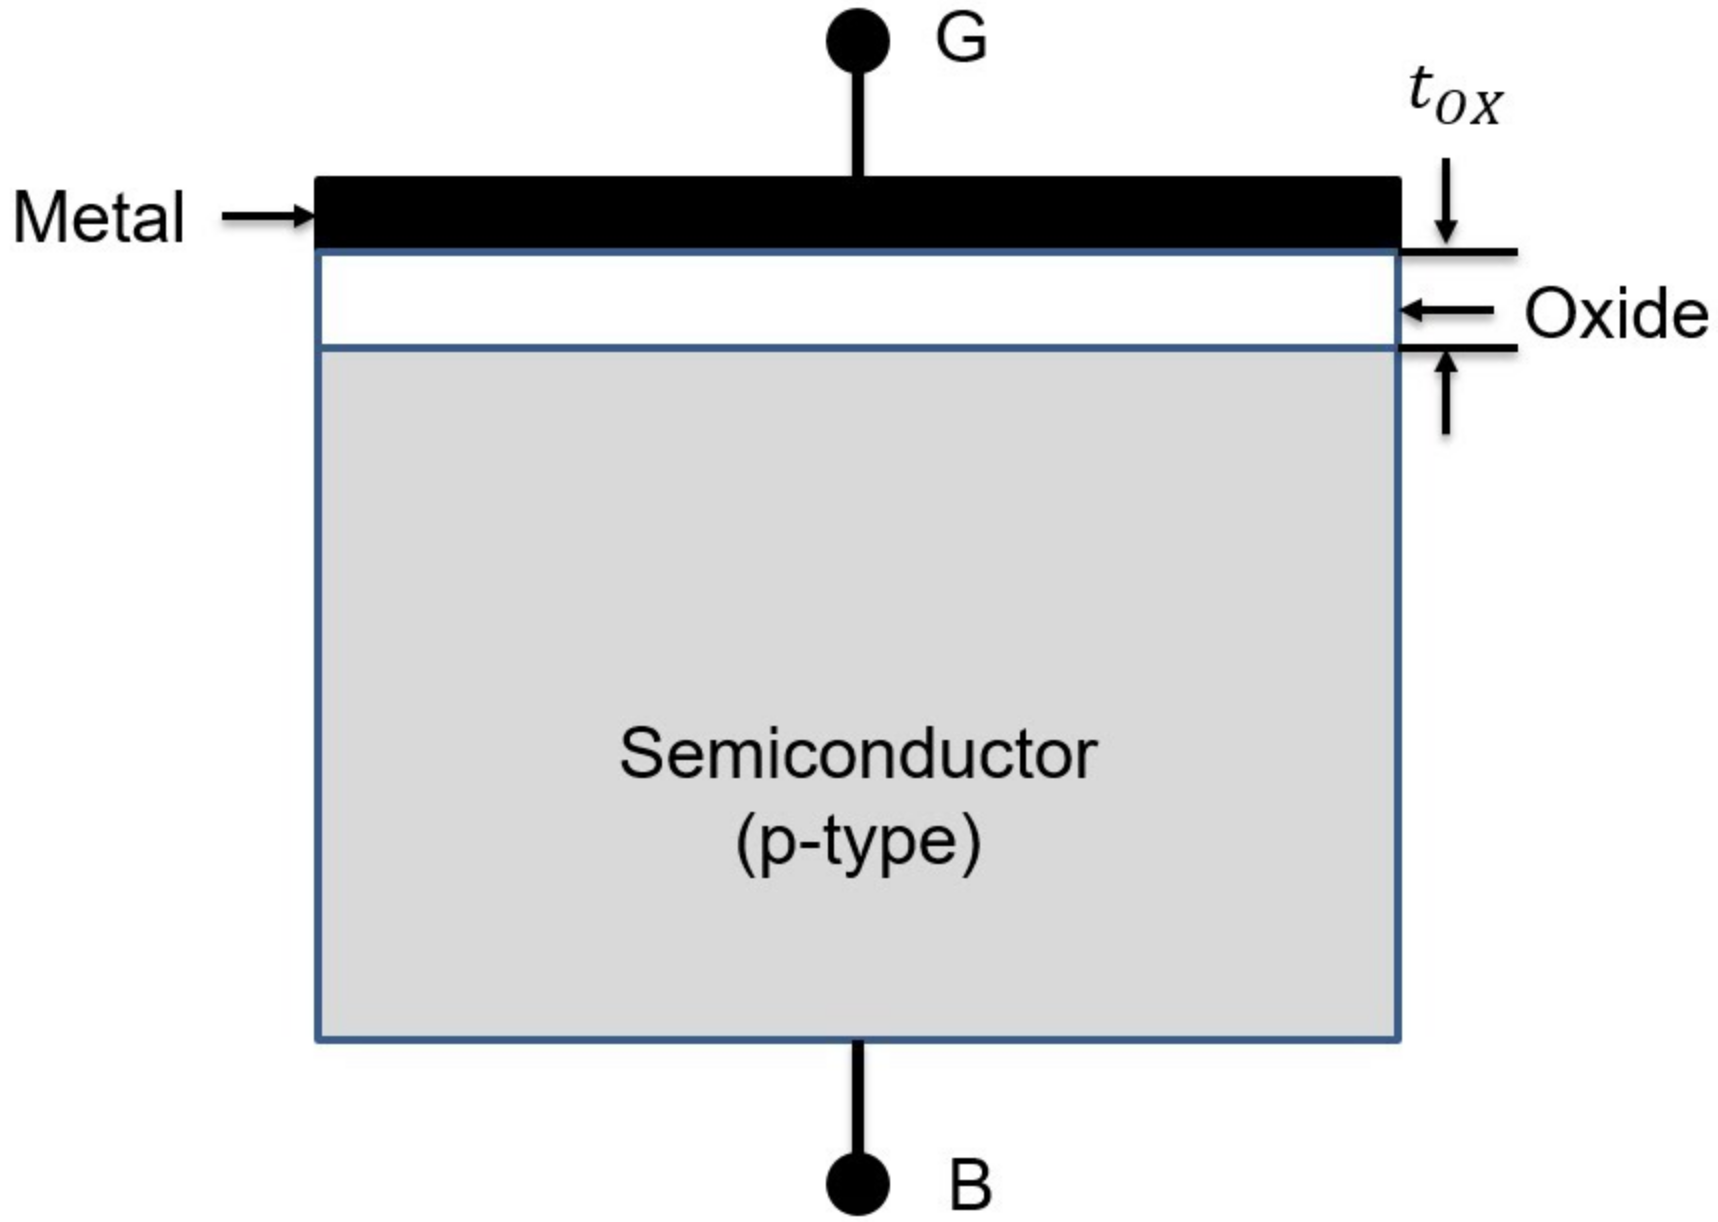
\includegraphics[scale=0.18]{../figures/moscap.png}
\end{center}

Questo è composto da 3 strati:
\begin{enumerate}
	\item Uno strato base di semiconduttore drogato, che solitamente è il \textit{silicio} ($Si$) drogato P. Questo fa da armatura del condensatore;
	\item Uno strato intermedio di \textit{ossido}, che storicamente era l'\textit{ossido di silicio} ($Si O_2$). Noi, in generale, assumiamo che l'ossido è un isolante perfetto (nella realtà non lo è mai, ma questa approssimazione ci è utile). Questo fa da dielettrico del condensatore;
	\item Uno strato superiore \textit{metallico}, che storicamente era l'\textit{aluminio} ($Al$). Anche questo, chiaramente, fa da armatura.
\end{enumerate}

La motivazione dietro l'uso del silicio e il suo ossido è stata storicamente la facile reperibilità del primo (la silice è ampiamente disponibile in natura) e la facile realizzazione del secondo (basta scaldare il silicio ed esporlo a ossigeno o vapore acqueo per realizzare uno strato di ossido). Oggi, anziché l'aluminio, si usa il \textit{polisilicio}, che è un silicio riarrangiato per rimuoverne la struttura cristallina, fortemente drogato. 

Prendiamo quindi il substrato di silicio e colleghiamolo a massa, e colleghiamo lo strato di alluminio ad un generatore di tensione $V_G$.

Vediamo quindi il comportamento del MOSCAP al variare di $V_G$:
\begin{enumerate}
\item $V_G < 0$ \\
In questo caso, applicando tensione negativa allo strato metallico, si crea un campo elettrico rivolto dal substrato (a massa) allo strato metallico stesso. Si ha quindi un accumulo di cariche negative sullo strato metallico, che a loro volta attirano i portatori di carica positiva (le lacune) dal substrato. 

Riguardo alle densità di portatori di carica positivi, si avrà:
$$
p_\text{superficiale} >> p_\text{substrato}
$$
e diremo di essere in \textbf{accumulazione} (in quanto le lacune del substrato si spostano verso la superficie, accumulandosi).

\item $V_G > 0$ \\
In questo caso, applicando tensione positiva allo strato metallico, si crea un campo elettrico rivolto dallo strato metallico stesso al substrato. Si ha quindi un accumulo di cariche positive sullo strato metallico, che a loro volta attirano i portatori di carica negativa dal substrato. 

Potremmo dire che questi portatori sono gli elettroni. Abbiamo però che la risposta non è totalmente giusta (di base gli elettroni nel silicio P sono pochi), in quanto in verità si forma una \textit{zona di svuotamento} fra il substrato e l'ossido. I portatori negativi sono quindi gli ioni fissi che restano nella regione superiore del substrato.

Riguardo alle densità di portatori di carica positivi, si avrà:
$$
p_\text{superficiale} << p_\text{substrato}
$$
e diremo di essere in \textbf{svuotamento}.

\item $V_G > V_T$ \\
Cose particolari accadono quanto la tensione $V_G$ supera una certa $V_T$ detta \textit{tensione di soglia} o \textit{threshold}. Notiamo che questa \textit{non va assolutamente confusa} con la tensione termica $V_T$, ovvero adesso:
$$
V_T \neq 26 \, \mathrm{mV} \ (\text{!!!})
$$

In questo caso gli elettroni liberi del substrato, che ricordiamo sono dati dalla legge di massa  azione:
$$
n = \frac{n_i^2}{p}
$$
e quindi sono pochi, vanno a disporsi in un sottile strato al di sopra degli ioni fissi della zona di svotamento.

Possiamo quindi definire $V_T$, per l'esattezza, come la tensione alla quale la concentrazione degli elettroni in superficie è uguale alla concentrazione delle lacune nel substrato. In simboli si ha:
$$
n_S^* = P_\text{substrato}
$$

Considerando la sola porzione dove è avvenuto questo fenomeno, cioè lo strato sottile di elettroni liberi, si è ottenuta effettivamente una regione di tipo N nel silicio di tipo P. Diciamo anche di aver raggiunto la cosiddetta \textbf{inversione}.

Ciò che accade di preciso è che solo la zona immediatamente inferiore all'elettrodo $G$ che applica il voltaggio $V_G$ si ha il fenomeno di inversione. La differenza nel FET sarà che manterremo due \textit{serbatoi} di elettroni a destra e a sinistra dell'elettrodo in modo da rendere costante lo strato di elettroni.

\end{enumerate}

\subsubsection{Modello fisico del transistore}
Veniamo quindi a vedere nello specifico la struttura ed una modellizzazione del transistore MOSFET.

\begin{center}
	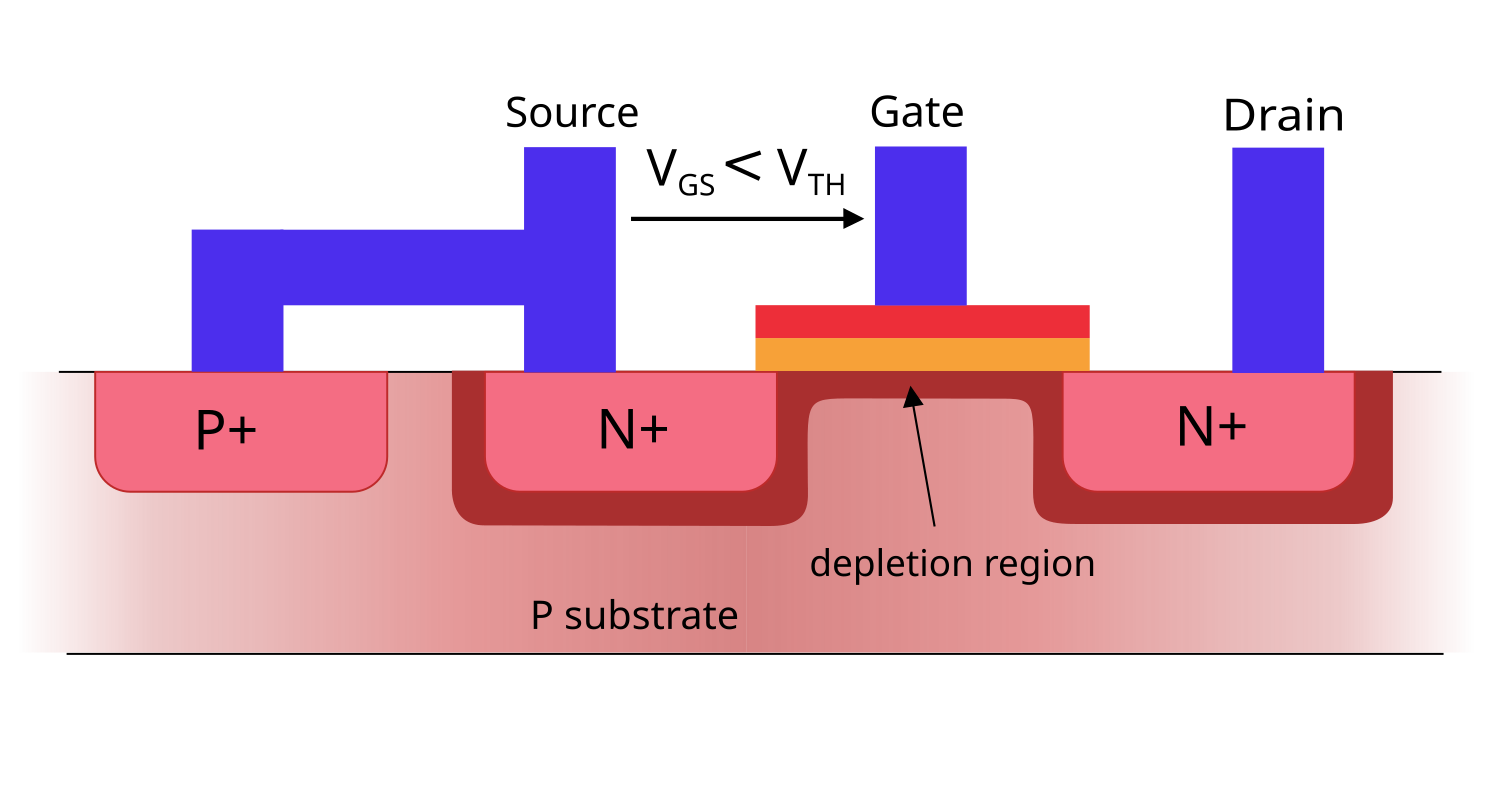
\includegraphics[scale=1]{../figures/mosfet.png}
\end{center}

Questo sarà dato, come per il MOSCAP, da 3 strati sovrapposti:
\begin{enumerate}
	\item Uno strato base di semiconduttore drogato, che solitamente è il \textit{silicio} ($Si$) drogato P;
	\item Uno strato intermedio di \textit{ossido}, che storicamente era l'\textit{ossido di silicio} ($Si O_2$). Noi, in generale, assumiamo che l'ossido è un isolante perfetto (nella realtà non lo è mai, ma questa approssimazione ci è utile);
	\item Uno strato superiore \textit{metallico}, che storicamente era l'\textit{aluminio} ($Al$).
\end{enumerate}

La differenza dal MOSCAP è data dal fatto che abbiamo 2 ulteriori elettrodi, collegati a regioni drogate N sul substrato P. Chiamiamo questi elettrodi \textit{source} \textit{drain}. A questo punto l'elettrodo $G$ che abbiamo visto finora viene detto \textit{gate}. Notiamo che in alcune traduzioni si parla rispettivamente di \textit{sorgente}, \textit{pozzo} e \textit{porta} (o erroneamente \textit{base}).
Notiamo che anche il substrato stesso fa da elettrodo, che viene detto \textit{body} o \textit{corpo}, solitamente a massa.

Vediamo che fra il substrato di tipo P e i due elettrodi di tipo N (source e drain) si formano sostanzialmente dei diodi (chiamiamoli $D_1$ e $D_2$), che impediscono il passaggio di corrente da source e drain al substrato.

Per il funzionamento del MOSFET, quindi, abbiamo bisogno che le zone drogate N si vadano a sovrapporre (almeno leggermente) all'ossido. Chiamiamo la distanza $L$ fra le zone drogate N \textit{distanza di gate} o \textit{lunghezza di gate}.

\end{document}
